\documentclass[11pt]{article}

% ---------- Packages ----------
\usepackage[letterpaper,margin=0.9in]{geometry}
\usepackage{amsmath,amssymb}
\usepackage{array}
\usepackage{tabularx}
\usepackage{booktabs}
\usepackage{tikz}
\usepackage{pgfplots}
\pgfplotsset{compat=1.18}
\usetikzlibrary{calc,arrows.meta}
\usepackage{enumitem}
\usepackage{fancyhdr}
\usepackage{xcolor}
\usepackage{graphicx}
\usepackage{needspace}

% ---------- Page style ----------
\pagestyle{fancy}
\fancyhf{}
\fancyhead[L]{\textit{enVision}\textsuperscript{\textregistered} Algebra 2}
\fancyhead[R]{Topic 5 Performance Assessment --- Form B}
\fancyfoot[C]{\thepage}
\renewcommand{\headrulewidth}{0.4pt}

\setlength{\parindent}{0pt}
\setlength{\parskip}{0.5em}

% ---------- Reusable: pyramid figure ----------
% A rectangular-base pyramid with base 3x by 2x and height x.
\newcommand{\PyramidFigure}{%
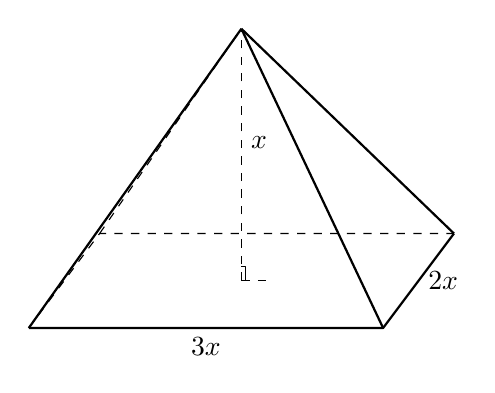
\begin{tikzpicture}[scale=1.0, line join=round]
  % Base corners (3x wide along bottom-front, 2x along side, using a slight
  % oblique projection so the back edge appears receded).
  \coordinate (A) at (0,0);          % front-left
  \coordinate (B) at (4.5,0);        % front-right  (base length 3x)
  \coordinate (C) at (5.4,1.2);      % back-right   (base depth 2x, receded)
  \coordinate (D) at (0.9,1.2);      % back-left
  % Base center
  \coordinate (O) at ($(A)!0.5!(C)$);
  % Apex directly above center at height
  \coordinate (P) at ($(O)+(0,3.2)$);

  % Back (hidden) edges dashed
  \draw[dashed] (A) -- (D) -- (C);
  \draw[dashed] (D) -- (P);

  % Visible base edges
  \draw[thick] (A) -- (B) -- (C);

  % Lateral edges to apex
  \draw[thick] (A) -- (P);
  \draw[thick] (B) -- (P);
  \draw[thick] (C) -- (P);

  % Height from center of base to apex (dashed) + small right-angle marker
  \draw[dashed] (O) -- (P);
  \draw[dashed] (O) -- ($(O)+(0.35,0)$); % short helper segment for right angle
  \draw ($(O)+(0.05,0)$) -- ($(O)+(0.05,0.18)$) -- ($(O)+(0,0.18)$);

  % Labels
  \node[below] at ($(A)!0.5!(B)$) {$3x$};          % front base edge
  \node[right] at ($(B)!0.5!(C)$) {$2x$};          % right base edge
  \node[right] at ($(O)!0.55!(P)$) {$x$};          % height
\end{tikzpicture}%
}

% ---------- Reusable: blank graph grid for Item 2 ----------
\newcommand{\BlankGraph}{%
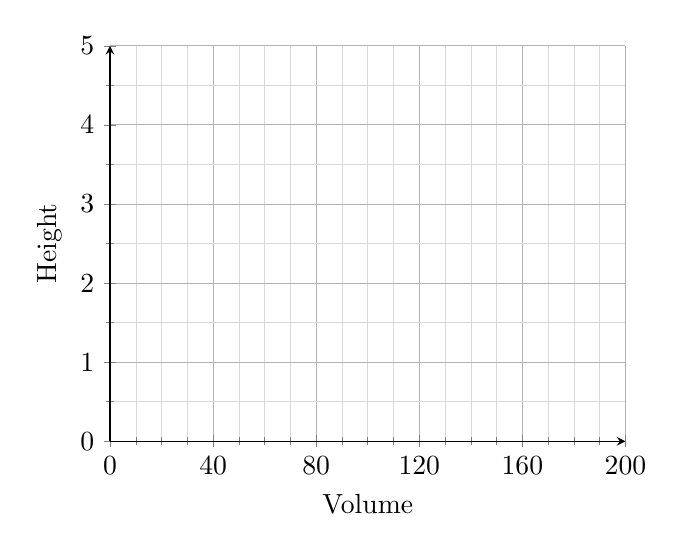
\begin{tikzpicture}
  \begin{axis}[
    width=3.2in, height=2.6in,
    xmin=0, xmax=200, ymin=0, ymax=5,
    xtick={0,40,80,120,160,200},
    ytick={0,1,2,3,4,5},
    xlabel={Volume},
    ylabel={Height},
    grid=both,
    major grid style={line width=.3pt,draw=gray!60},
    minor grid style={line width=.2pt,draw=gray!30},
    minor x tick num=3,
    minor y tick num=1,
    axis lines=left,
  ]
  \end{axis}
\end{tikzpicture}%
}

% ---------- Reusable: answer graph with curve ----------
\newcommand{\AnswerGraph}{%
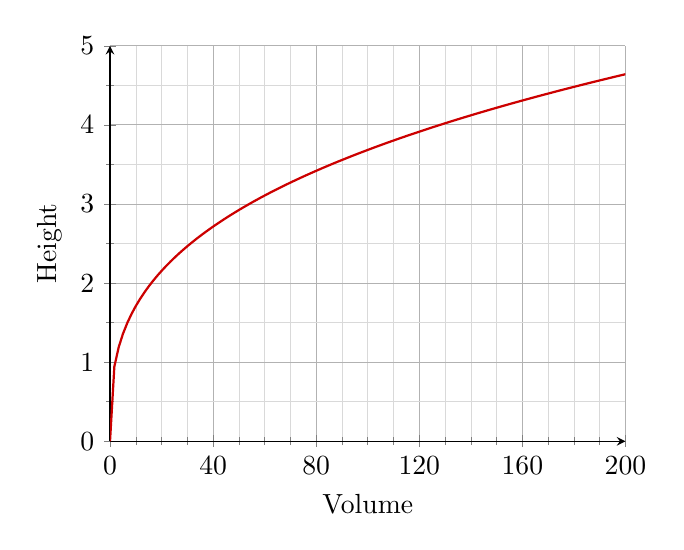
\begin{tikzpicture}
  \begin{axis}[
    width=3.2in, height=2.6in,
    xmin=0, xmax=200, ymin=0, ymax=5,
    xtick={0,40,80,120,160,200},
    ytick={0,1,2,3,4,5},
    xlabel={Volume},
    ylabel={Height},
    grid=both,
    major grid style={line width=.3pt,draw=gray!60},
    minor grid style={line width=.2pt,draw=gray!30},
    minor x tick num=3,
    minor y tick num=1,
    axis lines=left,
    samples=120, domain=0:200,
  ]
    % x = (4V)^(1/3) / 2
    \addplot[thick, red!80!black] { (4*x)^(1/3) / 2 };
  \end{axis}
\end{tikzpicture}%
}

% =====================================================================
\begin{document}

% ---------- Name / title block ----------
\noindent\textbf{Name} \hrulefill\hspace{2em}\textit{SavvasRealize.com}

\vspace{0.5em}
{\LARGE\textbf{5\quad Performance Assessment \quad Form B}}

\vspace{1.2em}

% ---------- Item 1 (problem setup + figure) ----------
\begin{minipage}[t]{0.62\textwidth}
\vspace{0pt}
According to a popular, but untrue, urban legend, oceanographers have
discovered images of giant pyramids made of crystal-like substances deep in
the ocean. Suppose one of these imaginary pyramids has the dimensions shown
at the right.

\vspace{0.6em}
\textbf{1.} The volume $V$ of a pyramid is $\dfrac{1}{3}Bh$, where $B$ is the
area of the base and $h$ is the height of the pyramid.
\end{minipage}\hfill
\begin{minipage}[t]{0.34\textwidth}
\vspace{0pt}
\centering
\PyramidFigure
\end{minipage}

\vspace{0.8em}
\textbf{Part A}

Find an equation that represents $V$ in terms of $x$. Then find $x$ in terms
of $V$. Write your equation for $x$ in rational exponent form, and
rationalize denominators where necessary. Explain.

\vspace{5em}

\textbf{Part B}

Suppose the urban legend were true, and a contractor could be hired to raise
one of these pyramids and bring it to the surface of the ocean. The
estimated cost of the operation $c(x)$ is \$200{,}000 per meter of pyramid
height, with an additional cost $a(V)$ of \$300 per cubic meter of pyramid
volume. Suppose a pyramid has a volume of $2{,}000{,}000\ \text{m}^3$. What is
the height $x$ of the pyramid? What is an equation that represents the total
retrieval cost $t$ for a pyramid of any volume with these proportions in
terms of $x$? How much would it cost to excavate this pyramid? Explain.

\vspace{8em}

\newpage

% ---------- Item 2 ----------
\textbf{2.} Complete the table that relates the pyramid's height to its volume.
Then graph the equation $x = \dfrac{(4V)^{\tfrac{1}{3}}}{2}$. Where necessary,
round values to the nearest tenth.

\vspace{0.8em}
\begin{minipage}[c]{0.38\textwidth}
\centering
\renewcommand{\arraystretch}{1.35}
\begin{tabular}{|>{\centering\arraybackslash}m{1.4cm}|>{\centering\arraybackslash}m{1.8cm}|}
\hline
\textbf{Volume ($V$)} & \textbf{Height ($x$)} \\
\hline
0    & \phantom{0.0} \\ \hline
0.25 & \phantom{0.0} \\ \hline
2    & \phantom{0.0} \\ \hline
16   & \phantom{0.0} \\ \hline
32   & \phantom{0.0} \\ \hline
64   & \phantom{0.0} \\ \hline
128  & \phantom{0.0} \\ \hline
\end{tabular}
\end{minipage}\hfill
\begin{minipage}[c]{0.58\textwidth}
\centering
\BlankGraph
\end{minipage}

\vspace{2em}

% ---------- Item 3 ----------
\textbf{3.} What is the inverse of the relation represented in the table in
Item 2? Complete the table of values.

\vspace{0.8em}
\begin{center}
\renewcommand{\arraystretch}{1.35}
\begin{tabular}{|>{\centering\arraybackslash}m{2cm}|>{\centering\arraybackslash}m{2cm}|}
\hline
\textbf{Height ($x$)} & \textbf{Volume ($V$)} \\
\hline
\phantom{0.0} & \phantom{0.00} \\ \hline
\phantom{0.0} & \phantom{0.00} \\ \hline
\phantom{0.0} & \phantom{0.00} \\ \hline
\phantom{0.0} & \phantom{0.00} \\ \hline
\phantom{0.0} & \phantom{0.00} \\ \hline
\phantom{0.0} & \phantom{0.00} \\ \hline
\phantom{0.0} & \phantom{0.00} \\ \hline
\end{tabular}
\end{center}

\vfill
\begin{center}\footnotesize
\textit{enVision}\textsuperscript{\textregistered} Algebra 2 \quad\textbullet\quad
Assessment Sourcebook \quad\textbullet\quad
Copyright \textcopyright{} Savvas Learning Company LLC. All Rights Reserved.
\end{center}

% =====================================================================
\newpage
% ---------- Teacher Answer Key ----------
\begin{center}
{\Large\textbf{Teacher Answer Key --- Topic 5 Performance Assessment, Form B}}
\end{center}

\vspace{0.8em}

\textbf{1. Part A.}\quad Find $V$ in terms of $x$, then $x$ in terms of $V$.

The base is a rectangle with sides $3x$ and $2x$, so
\[
B = (3x)(2x) = 6x^2, \qquad h = x.
\]
Therefore
\[
V = \tfrac{1}{3}Bh = \tfrac{1}{3}(6x^2)(x) = 2x^3.
\]

Solving for $x$:
\[
V = 2x^3 \;\Longrightarrow\; x^3 = \frac{V}{2}
\;\Longrightarrow\; x = \sqrt[3]{\frac{V}{2}}
= \frac{\sqrt[3]{V}}{\sqrt[3]{2}}.
\]
Rationalize by multiplying numerator and denominator by $\sqrt[3]{2^2}$:
\[
x = \frac{\sqrt[3]{V}}{\sqrt[3]{2}}\cdot\frac{\sqrt[3]{2^2}}{\sqrt[3]{2^2}}
= \frac{\sqrt[3]{4V}}{2}
= \boxed{\,\frac{(4V)^{\tfrac{1}{3}}}{2}\,}.
\]

\vspace{0.4em}
\textbf{1. Part B.}\quad Height, total cost function, and cost for $V=2{,}000{,}000\ \text{m}^3$.

From $V = 2x^3$:
\[
2{,}000{,}000 = 2x^3 \;\Longrightarrow\; x^3 = 1{,}000{,}000
\;\Longrightarrow\; x = \sqrt[3]{1{,}000{,}000} = 100\ \text{m}.
\]

Build the total cost $t(x)$ from the two pieces:
\begin{align*}
a(V) &= 300\cdot V = 300(2x^3) = 600x^3, \\
c(x) &= 200{,}000x, \\
t(x) &= c(x) + a(V) = 200{,}000x + 600x^3.
\end{align*}

Evaluate at $x = 100$:
\[
t(100) = 200{,}000(100) + 600(100)^3
       = 20{,}000{,}000 + 600{,}000{,}000
       = \boxed{\$620{,}000{,}000}.
\]

\vspace{1.2em}

\textbf{2.}\quad Completed table and graph of $x = \dfrac{(4V)^{1/3}}{2}$.

\begin{minipage}[c]{0.38\textwidth}
\centering
\renewcommand{\arraystretch}{1.3}
\begin{tabular}{|>{\centering\arraybackslash}m{1.4cm}|>{\centering\arraybackslash}m{1.8cm}|}
\hline
\textbf{Volume ($V$)} & \textbf{Height ($x$)} \\ \hline
0    & 0   \\ \hline
0.25 & 0.5 \\ \hline
2    & 1   \\ \hline
16   & 2   \\ \hline
32   & 2.5 \\ \hline
64   & 3.2 \\ \hline
128  & 4   \\ \hline
\end{tabular}
\end{minipage}\hfill
\begin{minipage}[c]{0.58\textwidth}
\centering
\AnswerGraph
\end{minipage}

\vspace{1em}

\textbf{3.}\quad Inverse of the relation in Item 2 (swap the columns):

\begin{center}
\renewcommand{\arraystretch}{1.3}
\begin{tabular}{|>{\centering\arraybackslash}m{2cm}|>{\centering\arraybackslash}m{2cm}|}
\hline
\textbf{Height ($x$)} & \textbf{Volume ($V$)} \\ \hline
0    & 0    \\ \hline
0.5  & 0.25 \\ \hline
1    & 2    \\ \hline
2    & 16   \\ \hline
2.5  & 32   \\ \hline
3.2  & 64   \\ \hline
4    & 128  \\ \hline
\end{tabular}
\end{center}

\vspace{0.5em}
\textit{Note.} The inverse corresponds to $V = 2x^3$, which is the original
volume relation --- consistent with the fact that the equation in Item 2 was
obtained by solving $V = 2x^3$ for $x$.

\end{document}
